\section{Results}\label{sec:results}

\subsection{Network design across promises and speeds}

Table~\ref{tab:e1} and Figure~\ref{fig:price} report the cost-minimising networks (M1--M2) for every combination of promise $T$ and safe speed $v$. All instances solved to optimality with HiGHS. Three results stand out.

\begin{table}[ht]
\centering\small
\caption{Cost-minimising dark-store networks for Bengaluru (M1--M2). Cost per order is per \emph{served} order and includes store and rider costs.}\label{tab:e1}
\begin{tabular}{rrrrrrrr}
\toprule
$T$ & $v$ & Radius & Stores & Reachable & Riders & Orders/ & Cost/order \\
(min) & (km/h) & (km) & & pop.\ (\%) & (peak) & store/day & (INR) \\
\midrule
10 & 12 & 1.21 & 390 & 79.3 & 6,705 & 1,220 & 50.4 \\
10 & 15 & 1.51 & 320 & 86.7 & 6,902 & 1,626 & 43.4 \\
10 & 20 & 2.01 & 226 & 94.2 & 6,872 & 2,501 & 35.6 \\
15 & 12 & 2.21 & 270 & 95.9 & 10,295 & 2,130 & 49.3 \\
15 & 15 & 2.76 & 240 & 98.3 & 9,275 & 2,458 & 43.2 \\
15 & 20 & 3.68 & 203 & 99.8 & 7,929 & 2,950 & 36.3 \\
20 & 12 & 3.21 & 261 & 99.4 & 11,341 & 2,286 & 50.8 \\
20 & 15 & 4.01 & 239 & 99.9 & 9,700 & 2,509 & 43.9 \\
20 & 20 & 5.34 & 204 & 100.0 & 7,968 & 2,941 & 36.4 \\
30 & 12 & 5.21 & 260 & 100.0 & 11,553 & 2,308 & 51.2 \\
30 & 15 & 6.51 & 238 & 100.0 & 9,733 & 2,521 & 43.9 \\
30 & 20 & 8.68 & 202 & 100.0 & 7,987 & 2,970 & 36.4 \\
\bottomrule
\end{tabular}

\end{table}

\begin{figure}[ht]
\centering
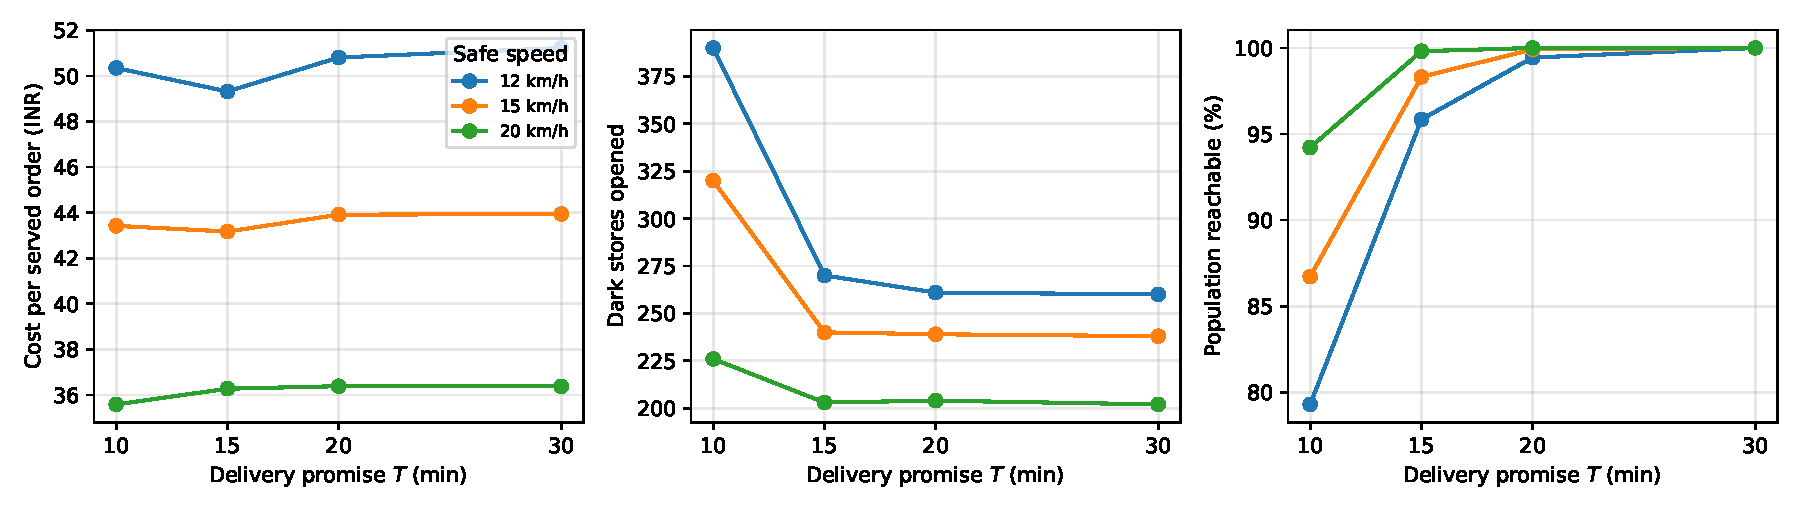
\includegraphics[width=\linewidth]{price_of_speed.pdf}
\caption{The price of speed: cost per served order, stores opened and share of residents reachable, by promise $T$ and safe rider speed $v$.}\label{fig:price}
\end{figure}

\paragraph{The promise decides \emph{who} is served, not what it costs.} At a safe speed of \BaseV~km/h, a 15-minute promise reaches \ServedFifteenPct\% of residents with \StoresTFifteen{} stores at INR~\CostPerOrderFifteen{} per order. Tightening to 10 minutes raises the store count to \StoresTTen{} but leaves \UnreachTenPct\% of residents---mostly at the city's edge, where retail stock suitable for dark stores is sparse---with no candidate site within reach (Figure~\ref{fig:maps}); the cost per served order barely moves (INR~\CostPerOrderTen{}). Relaxing the promise beyond 15 minutes changes almost nothing: the cost-optimal network has about \StoresTTwenty{} stores whether the promise is 20 or 30 minutes, because the cost trade-off between stores and rider time, not the promise, then determines the radius.

\paragraph{The speed cap decides what it costs.} Because riders are paid per logged-in hour, cost per order falls steeply with rider speed: at $T=15$ it is INR~\CostPerOrderVTwelve{} at 12~km/h, \CostPerOrderFifteen{} at 15~km/h and \CostPerOrderVTwenty{} at 20~km/h. Capping speed at 15 rather than 20~km/h costs about \SpeedCapPremiumPct\% more per order. This is the platform's economic incentive to push speed---independent of the advertised promise---and the quantity a regulator implicitly prices when it sets a speed norm.

\paragraph{The cost-optimal network is smaller than today's.} A single network serving all of Bengaluru's demand at minimum cost needs \StoreRange{} stores across the scenarios, against roughly \CurrentStores{} operated by three competing platforms today. The gap is a measure of the duplication that competition creates.

\begin{figure}[ht]
\centering
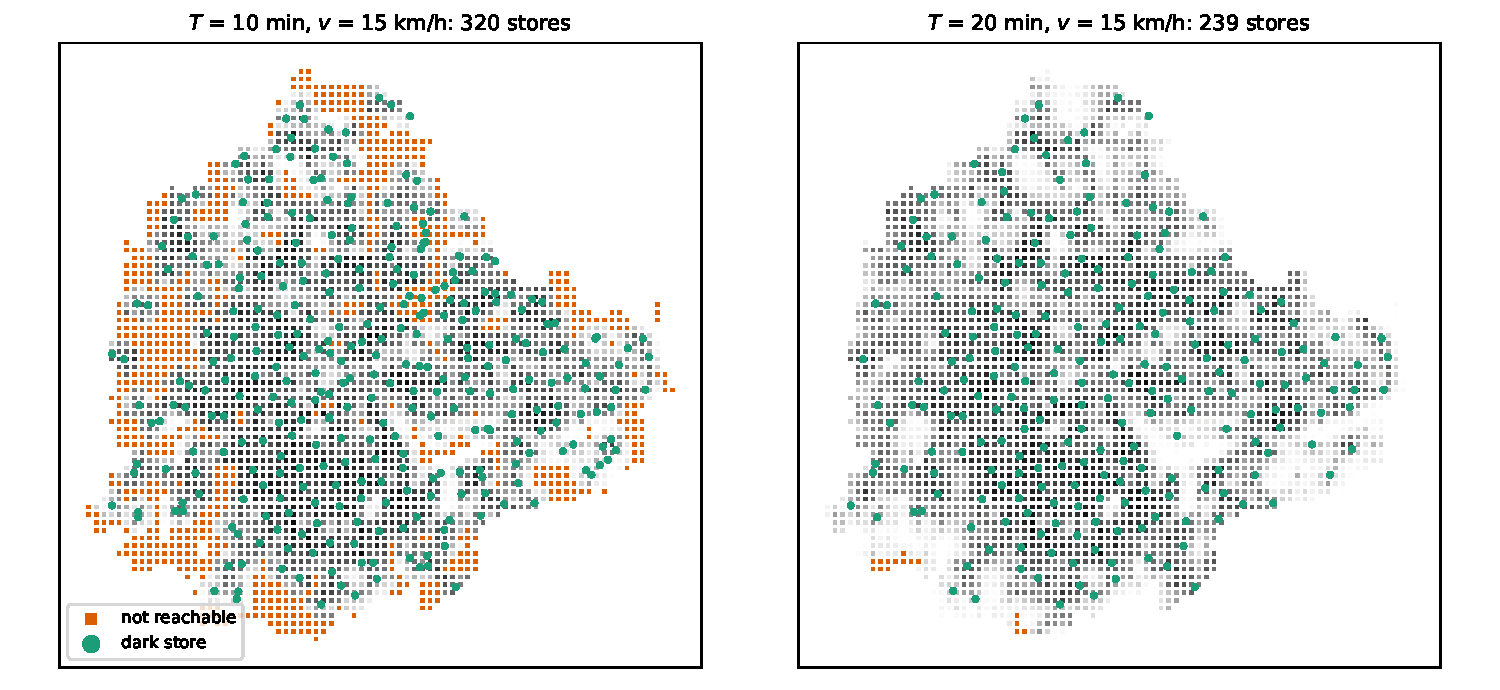
\includegraphics[width=\linewidth]{network_maps.pdf}
\caption{Optimal networks for $T=10$ and $T=20$ minutes at 15~km/h. Grey cells are served; orange cells have no candidate site within reach.}\label{fig:maps}
\end{figure}

\paragraph{The price of speed at equal coverage.} The coverage gap at $T=10$ arises because mapped retail sites are scarce at the city's edge. Allowing a store anywhere on a $\sim$0.9~km lattice of populated cells (\GridCandidates{} candidate sites), a 10-minute promise reaches \GridTenServedPct\% of residents but needs \GridTenStores{} stores at INR~\GridTenCost{} per order, against \GridFifteenStores{} stores at INR~\GridFifteenCost{} for 15 minutes. Serving \emph{everyone} within 10 rather than 15 minutes therefore needs \GridStorePremiumPct\% more stores and costs \GridCostPremiumPct\% more per order---about INR~\GridPricePerMinute{} per order for each minute saved. The price of the last five minutes is paid mainly in real estate at the periphery, which the platforms' current networks largely avoid.

\subsection{Fulfilment reliability (PERT)}

Table~\ref{tab:pert} gives the PERT estimate of fulfilment time in each network at 15~km/h. Inside the designed networks every served address is within the ride radius, so on-time probabilities are high: \PertTenP\% at $T=10$. A 10-minute promise met 95\% of the time requires riders to average \PertTenSpeed~km/h in the 10-minute network---below the safe speed. Ten-minute delivery is therefore feasible without speeding, \emph{but only} with a dense network and only for the \ServedTenPct\% of residents that network can reach.

\begin{table}[ht]
\centering\small
\caption{PERT fulfilment time by promise (network designed for that promise, $v=15$~km/h).}\label{tab:pert}
\begin{tabular}{rrrrr}
\toprule
$T$ (min) & Mean (min) & SD (min) & $P$(on time) & Speed for 95\% (km/h) \\
\midrule
10 & 7.33 & 0.99 & 0.997 & 12.1 \\
15 & 8.11 & 1.31 & 1.000 & 8.3 \\
20 & 8.23 & 1.40 & 1.000 & 6.0 \\
30 & 8.23 & 1.40 & 1.000 & 5.0 \\
\bottomrule
\end{tabular}

\end{table}

\subsection{Peak dispatch (assignment)}

The pressure appears when a network designed for one promise is asked to meet a tighter one. Table~\ref{tab:assign} dispatches a 10-minute peak batch at a stressed store of the 15-minute network (90th percentile of mean ride distance, \AssignStressRide~km). With the full sized fleet, a 15-minute promise is met for every order, but a 10-minute promise only for \AssignStressTenOnTime\%; the late orders could be saved only if riders averaged about \AssignStressSpeed~km/h, above the safe speed. Under lean staffing the gap widens sharply. Optimal assignment reduces total lateness relative to first-in-first-out dispatch, although because it minimises lateness rather than the count of late orders it occasionally delivers fewer orders strictly on time. \todo{Comment on the median store, where 60\% staffing suffices for all promises.}

\begin{table}[ht]
\centering\small
\caption{Peak 10-minute batch at a stressed store of the 15-minute network: optimal assignment vs FIFO.}\label{tab:assign}
\begin{tabular}{rrrrrr}
\toprule
Staffing & Riders & $T$ & On time & On time & Mean lateness (min) \\
 & & (min) & optimal & FIFO & optimal / FIFO \\
\midrule
40\% & 32 & 10 & 17\% & 26\% & 4.24 / 4.47 \\
40\% & 32 & 15 & 56\% & 59\% & 0.89 / 1.46 \\
40\% & 32 & 20 & 100\% & 90\% & 0.00 / 0.25 \\
60\% & 47 & 10 & 35\% & 49\% & 1.19 / 1.52 \\
60\% & 47 & 15 & 100\% & 93\% & 0.00 / 0.10 \\
60\% & 47 & 20 & 100\% & 100\% & 0.00 / 0.00 \\
80\% & 63 & 10 & 64\% & 64\% & 0.82 / 0.83 \\
80\% & 63 & 15 & 100\% & 100\% & 0.00 / 0.00 \\
80\% & 63 & 20 & 100\% & 100\% & 0.00 / 0.00 \\
100\% & 79 & 10 & 64\% & 64\% & 0.82 / 0.82 \\
100\% & 79 & 15 & 100\% & 100\% & 0.00 / 0.00 \\
100\% & 79 & 20 & 100\% & 100\% & 0.00 / 0.00 \\
\bottomrule
\end{tabular}

\end{table}

\subsection{Replenishment (transportation)}

For the base network ($T=15$, $v=15$; \StoresTFifteen{} stores), replenishment from three equal-capacity mother hubs costs \TransLP~million order-km per day at the optimum. Vogel's approximation comes within \TransVAMGapPct\% of the optimum, while the north-west corner rule is \TransNWRatio{} times worse. Supplying each store from its nearest hub would cost \TransNearest~million order-km, so equal hub capacities carry a \TransCapPremiumPct\% premium. Because the store count hardly changes beyond 15 minutes, replenishment cost is insensitive to the promise in that range.

\subsection{Sensitivity analysis}

Figure~\ref{fig:tornado} varies each uncertain input over its range at the base case. The cost per order is most sensitive to \TornadoTop{} (a swing of INR~\TornadoTopSpan) and \TornadoSecond{} (INR~\TornadoSecondSpan): rider time dominates the cost structure, which is why speed is the platform's main lever. Higher rider cost or demand raises the optimal number of stores, shortening rides; higher store cost lowers it. Longer pick-and-pack times shrink the ride radius; cost per \emph{served} order changes little because the hardest-to-serve cells drop out, which again shows that tighter time budgets are paid in coverage. The headline findings---a store count near the base case, cost flat in $T$ beyond 15 minutes, and speed as the cost driver---hold across all ranges.

\begin{figure}[ht]
\centering
\IfFileExists{figures/tornado.pdf}{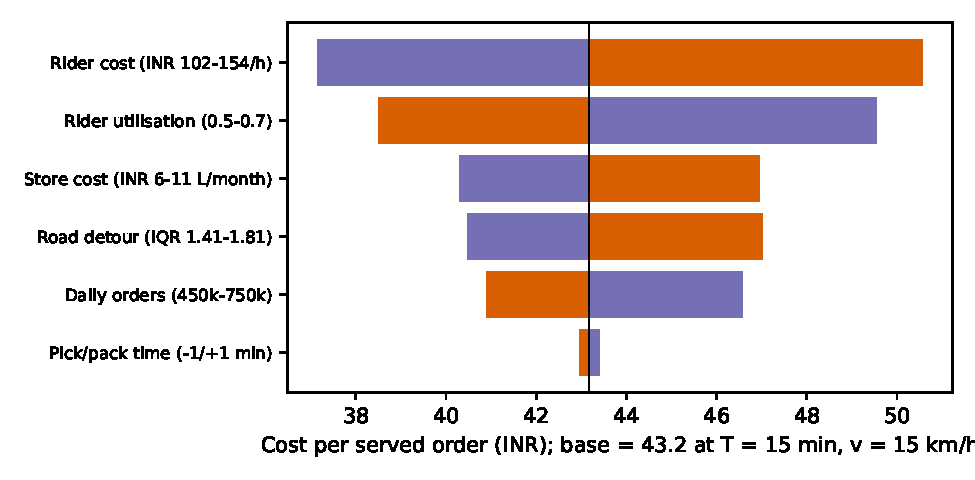
\includegraphics[width=0.85\linewidth]{tornado.pdf}}{\todo{tornado figure pending}}
\caption{One-at-a-time sensitivity of cost per served order ($T=15$, $v=15$).}\label{fig:tornado}
\end{figure}
